\documentclass[11pt]{article}
\usepackage[margin=1in]{geometry}
\usepackage{tikz}
\usetikzlibrary{shapes.geometric, arrows.meta, positioning, fit, backgrounds, calc}
\usepackage{booktabs}
\usepackage{enumitem}
\usepackage{hyperref}
\usepackage{listings}
\usepackage{xcolor}

\lstset{
    basicstyle=\ttfamily\small,
    breaklines=true,
    frame=single,
    backgroundcolor=\color{gray!10}
}

\title{Security Block Architecture Documentation}
\author{}
\date{\today}

\begin{document}

\maketitle
\tableofcontents
\newpage

%============================================================================
\section{Purpose}
%============================================================================

The security block implements a hardware-level ``deadman's switch'' for AI accelerators, as described in Petrie's ``Embedded Off-Switches for AI Compute'' paper. The block gates essential chip operations, allowing them to proceed only when valid, cryptographically-signed authorization has been recently received.

\subsection{Design Goals}

\begin{itemize}
    \item \textbf{Fail-secure default}: Output is blocked unless explicitly authorized
    \item \textbf{Cryptographic authorization}: Only holders of the private key can generate valid licenses
    \item \textbf{Replay prevention}: Each license is valid for exactly one nonce
    \item \textbf{Time-based depletion}: Authorization expires over time without renewal
\end{itemize}

%============================================================================
\section{High-Level Block Diagram}
%============================================================================

\begin{center}
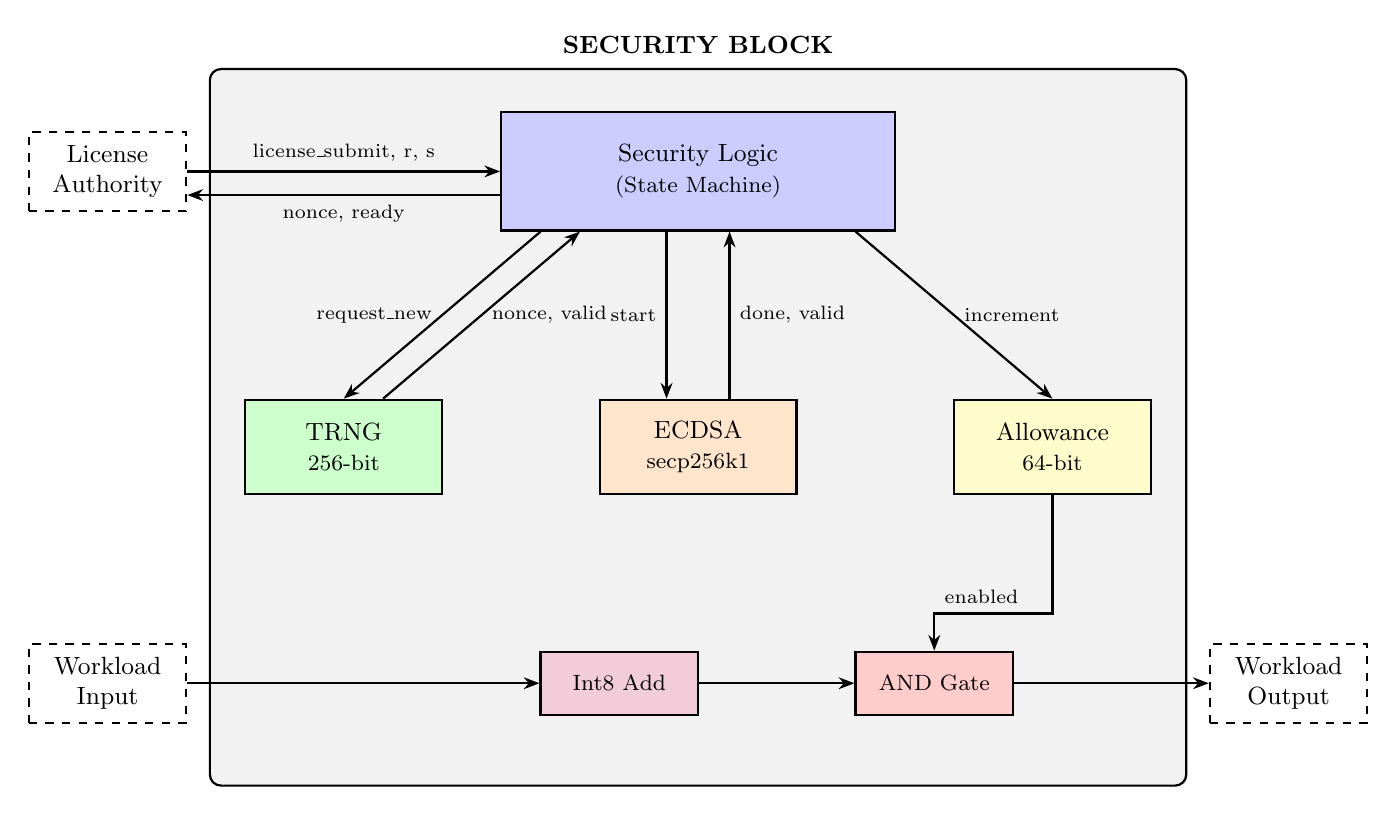
\begin{tikzpicture}[
    block/.style={rectangle, draw, thick, minimum width=2.5cm, minimum height=1.2cm, align=center, font=\small},
    smallblock/.style={rectangle, draw, thick, minimum width=2cm, minimum height=0.8cm, align=center, font=\footnotesize},
    external/.style={rectangle, draw, thick, dashed, minimum width=2cm, minimum height=1cm, align=center, font=\small},
    arrow/.style={-{Stealth[length=2mm]}, thick},
    label/.style={font=\scriptsize},
]

\node[block, fill=blue!20, minimum width=5cm, minimum height=1.5cm] (security) at (0, 0) 
    {Security Logic\\{\footnotesize (State Machine)}};

\node[block, fill=green!20] (trng) at (-4.5, -3.5) {TRNG\\{\footnotesize 256-bit}};
\node[block, fill=orange!20] (ecdsa) at (0, -3.5) {ECDSA\\{\footnotesize secp256k1}};
\node[block, fill=yellow!20] (allowance) at (4.5, -3.5) {Allowance\\{\footnotesize 64-bit}};

\node[smallblock, fill=purple!20] (adder) at (-1, -6.5) {Int8 Add};
\node[smallblock, fill=red!20] (andgate) at (3, -6.5) {AND Gate};

\node[external] (authority) at (-7.5, 0) {License\\Authority};
\node[external] (workload_in) at (-7.5, -6.5) {Workload\\Input};
\node[external] (workload_out) at (7.5, -6.5) {Workload\\Output};

\begin{scope}[on background layer]
    \draw[thick, rounded corners, fill=gray!10] 
        (-6.2, 1.3) rectangle (6.2, -7.8);
    \node[font=\small\bfseries] at (0, 1.6) {SECURITY BLOCK};
\end{scope}

\draw[arrow] ([xshift=-2cm]security.south) -- 
    node[label, left]{request\_new} (trng.north);
\draw[arrow] ([xshift=-0.4cm]security.south) -- 
    node[label, left]{start} ([xshift=-0.4cm]ecdsa.north);
\draw[arrow] ([xshift=2cm]security.south) -- 
    node[label, right]{increment} (allowance.north);
\draw[arrow] ([xshift=0.5cm]trng.north) -- 
    node[label, right]{nonce, valid} ([xshift=-1.5cm]security.south);
\draw[arrow] ([xshift=0.4cm]ecdsa.north) -- 
    node[label, right]{done, valid} ([xshift=0.4cm]security.south);
\draw[arrow] (allowance.south) -- ++(0, -1.5) -|
    node[label, above, pos=0.3]{enabled} (andgate.north);
\draw[arrow] (workload_in.east) -- (adder.west);
\draw[arrow] (adder.east) -- (andgate.west);
\draw[arrow] (andgate.east) -- (workload_out.west);
\draw[arrow] (authority.east) -- 
    node[label, above]{license\_submit, r, s} (security.west);
\draw[arrow] ([yshift=-0.3cm]security.west) -- 
    node[label, below]{nonce, ready} ([yshift=-0.3cm]authority.east);

\end{tikzpicture}
\end{center}

Security block architecture. The Int8 adder is a placeholder for actual chip operations (matrix multiplies, data routing, etc.).

\subsection{Module Summary}

\begin{table}[h]
\centering
\begin{tabular}{@{}llp{6cm}@{}}
\toprule
\textbf{Module} & \textbf{Type} & \textbf{Purpose} \\
\midrule
\texttt{Trng} & Submodule & Nonce generation (256-bit counter in prototype; ring oscillator in production) \\
\midrule
\texttt{Ecdsa} & Submodule & Signature verification using secp256k1 curve \\
\midrule
Security Logic & Inline & State machine orchestration (7 states) \\
\midrule
Usage Allowance & Inline & 64-bit authorization counter \\
\midrule
Workload & Inline & Gated essential operation (Int8 Add example) \\
\bottomrule
\end{tabular}
\caption{Module summary}
\end{table}

%============================================================================
\section{Data Flow}
%============================================================================

\subsection{Authorization Flow}

\begin{enumerate}
    \item TRNG generates nonce (at initialization or after valid license)
    \item Security Logic latches and publishes nonce (\texttt{nonce\_ready} = 1)
    \item External authority reads nonce, signs it with private key
    \item Authority submits license $(r, s)$ via \texttt{license\_submit} pulse
    \item ECDSA verifies signature against nonce and hardcoded public key
    \item \textbf{If valid:}
    \begin{enumerate}
        \item Allowance incremented
        \item Return to step 1 (new nonce generated)
    \end{enumerate}
    \item \textbf{If invalid:}
    \begin{enumerate}
        \item Allowance unchanged
        \item Same nonce retained (allows retry with correct signature)
        \item Return to step 2
    \end{enumerate}
\end{enumerate}

\subsection{Workload Flow}

\begin{enumerate}
    \item Workload inputs (\texttt{int8\_a}, \texttt{int8\_b}) arrive with \texttt{workload\_valid} = 1
    \item Computation performed (Int8 addition, wrapping on overflow)
    \item Output gating: each result bit ANDed with \texttt{enabled} signal
    \begin{itemize}
        \item If \texttt{allowance} $> 0$: \texttt{enabled} = 1, result passes through
        \item If \texttt{allowance} $= 0$: \texttt{enabled} = 0, result forced to zero
    \end{itemize}
    \item Result registered and output on next cycle
\end{enumerate}

\textbf{Note:} Allowance decrements every clock cycle regardless of workload activity. This provides time-based authorization depletion.

%============================================================================
\section{Trust Model}
%============================================================================

\subsection{Trust Boundaries}

\textbf{Untrusted:}
\begin{itemize}
    \item External license authority communication channel
    \item Workload inputs
    \item All signals crossing the security block boundary
\end{itemize}

\textbf{Trusted:}
\begin{itemize}
    \item ECDSA verification logic
    \item Hardcoded public key (in ECDSA module)
    \item Allowance counter logic
    \item Output gating logic (AND gates)
    \item State machine transitions
    \item TRNG entropy source (ring oscillator in production)
\end{itemize}

\subsection{Trust Assumptions}

\begin{enumerate}
    \item The hardcoded public key corresponds to a private key held only by authorized parties.
    \item ECDSA (secp256k1) is cryptographically secure---an attacker cannot forge signatures without the private key.
    \item The TRNG produces non-repeating nonces, preventing replay attacks. (Predictability is not a concern; uniqueness is.)
    \item The hardware implementation faithfully reflects this RTL design (no manufacturing-time tampering).
\end{enumerate}

%============================================================================
\section{Security Properties}
%============================================================================

\begin{table}[h]
\centering
\begin{tabular}{@{}p{3.2cm}p{4.5cm}p{5.5cm}@{}}
\toprule
\textbf{Property} & \textbf{Description} & \textbf{Enforcement} \\
\midrule
Output Gating & Workload output is 0 when unauthorized & \texttt{result \& repeat(enabled, 8)} \\
\midrule
Cryptographic Authorization & Only valid signatures increment allowance & ECDSA verification before increment \\
\midrule
Replay Prevention & Each license valid for one nonce only & New nonce generated only after valid license accepted \\
\midrule
Time-Based Depletion & Authorization depletes continuously & Allowance decrements every clock cycle \\
\midrule
Fail-Secure Default & Allowance initializes to 0 on reset & Register default value; no license = no output \\
\midrule
Retry Allowed & Invalid signatures allow retry with same nonce & State returns to Publish without changing nonce \\
\midrule
No Double-Spend & Same license cannot be reused & Nonce changes immediately after valid license \\
\bottomrule
\end{tabular}
\caption{Security properties and enforcement mechanisms}
\end{table}

%============================================================================
\section{Interface Specification}
%============================================================================

\subsection{Top-Level Inputs}

\begin{table}[h]
\centering
\begin{tabular}{@{}llp{7cm}@{}}
\toprule
\textbf{Signal} & \textbf{Width} & \textbf{Description} \\
\midrule
\texttt{clock} & 1 & System clock \\
\texttt{clear} & 1 & Synchronous reset (active high) \\
\midrule
\texttt{license\_submit} & 1 & Pulse high for one cycle to submit license \\
\texttt{license\_r} & 256 & ECDSA signature $r$ component \\
\texttt{license\_s} & 256 & ECDSA signature $s$ component \\
\midrule
\texttt{workload\_valid} & 1 & Workload input data valid \\
\texttt{int8\_a} & 8 & Signed 8-bit operand A \\
\texttt{int8\_b} & 8 & Signed 8-bit operand B \\
\midrule
\texttt{param\_a} & 256 & ECDSA curve parameter $a$ (0 for secp256k1) \\
\texttt{param\_b3} & 256 & ECDSA curve parameter $3b$ (21 for secp256k1) \\
\midrule
\texttt{trng\_seed} & 256 & Seed value for TRNG (testing only) \\
\texttt{trng\_load\_seed} & 1 & Load seed into TRNG (testing only) \\
\bottomrule
\end{tabular}
\caption{Top-level input signals}
\end{table}

\subsection{Top-Level Outputs}

\begin{table}[h]
\centering
\begin{tabular}{@{}llp{7cm}@{}}
\toprule
\textbf{Signal} & \textbf{Width} & \textbf{Description} \\
\midrule
\texttt{nonce} & 256 & Current nonce value \\
\texttt{nonce\_ready} & 1 & Nonce is stable and ready for signing \\
\midrule
\texttt{int8\_result} & 8 & Gated workload output \\
\texttt{result\_valid} & 1 & Result output is valid \\
\midrule
\texttt{allowance} & 64 & Current allowance counter value \\
\texttt{enabled} & 1 & Allowance $> 0$ \\
\midrule
\texttt{state\_debug} & 4 & Current state machine state (debug) \\
\texttt{licenses\_accepted} & 16 & Count of valid licenses processed (debug) \\
\texttt{ecdsa\_busy} & 1 & ECDSA verification in progress (debug) \\
\bottomrule
\end{tabular}
\caption{Top-level output signals}
\end{table}

\subsection{TRNG Submodule Interface}

\begin{table}[h]
\centering
\begin{tabular}{@{}lllp{6cm}@{}}
\toprule
\textbf{Direction} & \textbf{Signal} & \textbf{Width} & \textbf{Description} \\
\midrule
Input & \texttt{clock} & 1 & System clock \\
Input & \texttt{clear} & 1 & Synchronous reset \\
Input & \texttt{enable} & 1 & Enable entropy counter \\
Input & \texttt{request\_new} & 1 & Pulse to latch new nonce \\
Input & \texttt{seed} & 256 & Seed value (testing only) \\
Input & \texttt{load\_seed} & 1 & Load seed (testing only) \\
\midrule
Output & \texttt{nonce} & 256 & Latched nonce value \\
Output & \texttt{nonce\_valid} & 1 & Nonce has been latched \\
\bottomrule
\end{tabular}
\caption{TRNG submodule interface}
\end{table}

\subsection{ECDSA Submodule Interface}

\begin{table}[h]
\centering
\begin{tabular}{@{}lllp{6cm}@{}}
\toprule
\textbf{Direction} & \textbf{Signal} & \textbf{Width} & \textbf{Description} \\
\midrule
Input & \texttt{clock} & 1 & System clock \\
Input & \texttt{clear} & 1 & Synchronous reset \\
Input & \texttt{start} & 1 & Pulse to begin verification \\
Input & \texttt{z} & 256 & Message hash (= nonce) \\
Input & \texttt{r} & 256 & Signature $r$ component \\
Input & \texttt{s} & 256 & Signature $s$ component \\
Input & \texttt{param\_a} & 256 & Curve parameter $a$ \\
Input & \texttt{param\_b3} & 256 & Curve parameter $3b$ \\
\midrule
Output & \texttt{done\_} & 1 & Verification complete (pulse) \\
Output & \texttt{valid} & 1 & Signature is valid \\
Output & \texttt{busy} & 1 & Verification in progress \\
\bottomrule
\end{tabular}
\caption{ECDSA submodule interface}
\end{table}

%============================================================================
\section{State Machine}
%============================================================================

\subsection{State Diagram}

\begin{center}
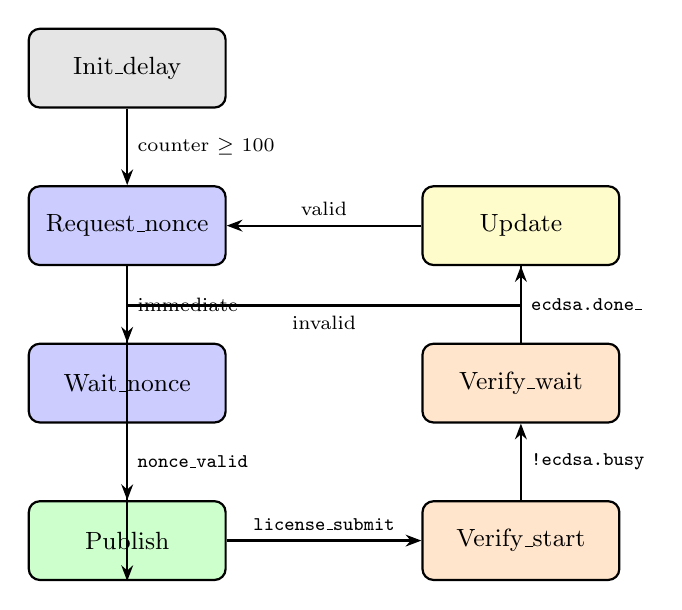
\begin{tikzpicture}[
    state/.style={rectangle, draw, thick, rounded corners, minimum width=2.5cm, minimum height=1cm, align=center, font=\small},
    arrow/.style={-{Stealth[length=2mm]}, thick},
    label/.style={font=\scriptsize},
]

\node[state, fill=gray!20] (init) at (0, 0) {Init\_delay};
\node[state, fill=blue!20] (request) at (0, -2) {Request\_nonce};
\node[state, fill=blue!20] (wait) at (0, -4) {Wait\_nonce};
\node[state, fill=green!20] (publish) at (0, -6) {Publish};
\node[state, fill=orange!20] (vstart) at (5, -6) {Verify\_start};
\node[state, fill=orange!20] (vwait) at (5, -4) {Verify\_wait};
\node[state, fill=yellow!20] (update) at (5, -2) {Update};

\draw[arrow] (init) -- node[label, right]{counter $\geq$ 100} (request);
\draw[arrow] (request) -- node[label, right]{immediate} (wait);
\draw[arrow] (wait) -- node[label, right]{\texttt{nonce\_valid}} (publish);
\draw[arrow] (publish) -- node[label, above]{\texttt{license\_submit}} (vstart);
\draw[arrow] (vstart) -- node[label, right]{\texttt{!ecdsa.busy}} (vwait);
\draw[arrow] (vwait) -- node[label, right]{\texttt{ecdsa.done\_}} (update);
\draw[arrow] (update.west) -- node[label, above]{valid} (request.east);
\draw[arrow] (update.south) -- ++(0, -0.5) -| node[label, below, pos=0.25]{invalid} (publish.south);

\end{tikzpicture}
\end{center}

\subsection{State Descriptions}

\begin{table}[h]
\centering
\begin{tabular}{@{}lp{3.5cm}p{4cm}p{3.5cm}@{}}
\toprule
\textbf{State} & \textbf{Entry Condition} & \textbf{Actions} & \textbf{Exit Condition} \\
\midrule
\texttt{Init\_delay} & Reset & Increment delay counter & Counter $\geq$ 100 \\
\midrule
\texttt{Request\_nonce} & From Init\_delay or Update (valid) & Assert \texttt{request\_new} to TRNG & Immediate \\
\midrule
\texttt{Wait\_nonce} & From Request\_nonce & Wait for TRNG & \texttt{nonce\_valid} \\
\midrule
\texttt{Publish} & From Wait\_nonce or Update (invalid) & Latch nonce; \texttt{nonce\_ready} = 1 & \texttt{license\_submit} \\
\midrule
\texttt{Verify\_start} & From Publish & Latch $r$, $s$; assert \texttt{ecdsa\_start} & \texttt{!ecdsa.busy} \\
\midrule
\texttt{Verify\_wait} & From Verify\_start & Wait for ECDSA & \texttt{ecdsa.done\_} \\
\midrule
\texttt{Update} & From Verify\_wait & If valid: increment allowance & Immediate \\
\bottomrule
\end{tabular}
\caption{State machine state descriptions}
\end{table}

%============================================================================
\section{Timing Characteristics}
%============================================================================

\begin{table}[h]
\centering
\begin{tabular}{@{}llp{7cm}@{}}
\toprule
\textbf{Operation} & \textbf{Cycles} & \textbf{Notes} \\
\midrule
Initialization delay & 100 & Configurable via \texttt{Config.init\_delay\_cycles} \\
\midrule
Nonce generation & 2 & Request + latch \\
\midrule
License verification & $\sim$1.5--2M & ECDSA scalar multiplication dominates \\
\midrule
Workload operation & 1 & Combinational add + output register \\
\midrule
Allowance per license & $10^{12}$ & Configurable via \texttt{Config.allowance\_increment} \\
\bottomrule
\end{tabular}
\caption{Timing characteristics}
\end{table}

\subsection{Allowance Calculation}

For a desired licensing period $T$ seconds at clock frequency $f$ Hz:

\[
\texttt{allowance\_increment} = T \times f
\]

\textbf{Examples at 1 GHz:}
\begin{itemize}
    \item 1 hour: $3600 \times 10^9 = 3.6 \times 10^{12}$
    \item 1 day: $86400 \times 10^9 = 8.64 \times 10^{13}$
    \item 1 week: $604800 \times 10^9 = 6.05 \times 10^{14}$
\end{itemize}

With 64-bit allowance counter, maximum value is $2^{64} - 1 \approx 1.8 \times 10^{19}$, supporting approximately 584 years at 1 GHz.

The current default of $10^{12}$ provides approximately 17 minutes of authorization per valid license at 1 GHz.

%============================================================================
\section{Test Coverage}
%============================================================================

\subsection{Test Cases}

\begin{table}[h]
\centering
\begin{tabular}{@{}clp{5.5cm}l@{}}
\toprule
\textbf{\#} & \textbf{Test Name} & \textbf{Description} & \textbf{Property} \\
\midrule
1 & Initial state & Allowance = 0, enabled = false & Fail-secure \\
\midrule
2 & Workload blocked & Output = 0 when allowance = 0 & Output gating \\
\midrule
3 & State machine & Reaches Publish state with valid nonce & State machine \\
\midrule
4 & Valid license & Allowance increments, accepted count increases & Crypto auth \\
\midrule
5 & Workload unblocked & Correct result after valid license & Output gating \\
\midrule
6 & Invalid license & Allowance unchanged, same nonce retained & Crypto auth, retry \\
\midrule
7 & Int8 positive & 50 + 30 = 80 & Workload \\
\midrule
8 & Int8 negative & -10 + -20 = -30 & Workload \\
\midrule
9 & Int8 mixed & 100 + -30 = 70 & Workload \\
\midrule
10 & Int8 wrapping & 127 + 1 = -128 & Workload \\
\midrule
11 & Allowance decrement & Decreases by 100 over 100 cycles & Time depletion \\
\midrule
12 & New nonce & Generated after valid license only & Replay prevention \\
\midrule
13 & Wrong nonce & License for different nonce rejected & Crypto auth \\
\midrule
14 & Replay attack & Same license rejected on second use & No double-spend \\
\bottomrule
\end{tabular}
\caption{Test cases and covered properties}
\end{table}

\subsection{Property Coverage Matrix}

\begin{table}[h]
\centering
\begin{tabular}{@{}lccccccccc@{}}
\toprule
\textbf{Property} & \textbf{T1} & \textbf{T2} & \textbf{T4} & \textbf{T5} & \textbf{T6} & \textbf{T11} & \textbf{T12} & \textbf{T13} & \textbf{T14} \\
\midrule
Output Gating & $\bullet$ & $\bullet$ & & $\bullet$ & & & & & \\
\midrule
Crypto Authorization & & & $\bullet$ & & $\bullet$ & & & $\bullet$ & $\bullet$ \\
\midrule
Replay Prevention & & & & & & & $\bullet$ & & $\bullet$ \\
\midrule
Time-Based Depletion & & & & & & $\bullet$ & & & \\
\midrule
Fail-Secure Default & $\bullet$ & $\bullet$ & & & & & & & \\
\midrule
Retry Allowed & & & & & $\bullet$ & & & & \\
\midrule
No Double-Spend & & & & & & & & & $\bullet$ \\
\bottomrule
\end{tabular}
\caption{Property coverage matrix}
\end{table}

%============================================================================
\section{Prototype Limitations}
%============================================================================

\begin{table}[h]
\centering
\begin{tabular}{@{}lll@{}}
\toprule
\textbf{Component} & \textbf{Prototype} & \textbf{Production} \\
\midrule
TRNG & 256-bit counter & Ring oscillator(s) with XORed entropy \\
\midrule
Hash function & Identity (nonce = message $z$) & SHA-256 \\
\midrule
Public key & Hardcoded ($Q = 2G$) & Configurable via ROM or fuses \\
\midrule
Curve & secp256k1 only & Multiple curves for redundancy \\
\midrule
Input validation & Minimal & Full range checking ($r, s \in [1, n-1]$) \\
\midrule
Side-channel & None & Constant-time operations \\
\bottomrule
\end{tabular}
\caption{Prototype vs production differences}
\end{table}

\subsection{Security Considerations for Production}

\begin{enumerate}
    \item \textbf{TRNG}: Replace counter with ring oscillator design. XOR multiple independent entropy sources for robustness against single-source failures or attacks.
    
    \item \textbf{Hash function}: Implement SHA-256 to hash nonce before use as ECDSA message. Current design uses nonce directly, which is acceptable for prototyping but not recommended for production.
    
    \item \textbf{Input validation}: Add range checking for signature components. Values $r$ and $s$ must be in range $[1, n-1]$ where $n$ is the curve order.
    
    \item \textbf{Side-channel resistance}: ECDSA implementation should use constant-time algorithms to prevent timing attacks. Consider power analysis countermeasures.
    
    \item \textbf{Formal verification}: State machine transitions and security properties should be formally verified to ensure no edge cases allow unauthorized operation.
    
    \item \textbf{Physical security}: Consider glitch detection, voltage monitoring, and physical shielding to protect against fault injection attacks.
\end{enumerate}

%============================================================================
\section{Configuration Parameters}
%============================================================================

\begin{lstlisting}[caption={Configuration parameters in security\_block.ml}]
module Config = struct
  let nonce_width = 256
  let signature_width = 256
  let allowance_width = 64
  let init_delay_cycles = 100
  let allowance_increment = 1_000_000_000_000  (* ~17 min at 1GHz *)
end
\end{lstlisting}

\begin{table}[h]
\centering
\begin{tabular}{@{}llp{6cm}@{}}
\toprule
\textbf{Parameter} & \textbf{Value} & \textbf{Description} \\
\midrule
\texttt{nonce\_width} & 256 & Width of nonce in bits (matches ECDSA message size) \\
\midrule
\texttt{signature\_width} & 256 & Width of signature components $r$ and $s$ \\
\midrule
\texttt{allowance\_width} & 64 & Width of allowance counter (supports $\sim$584 years at 1 GHz) \\
\midrule
\texttt{init\_delay\_cycles} & 100 & Cycles to wait after reset before requesting first nonce \\
\midrule
\texttt{allowance\_increment} & $10^{12}$ & Cycles added to allowance per valid license ($\sim$17 min at 1 GHz) \\
\bottomrule
\end{tabular}
\caption{Configuration parameter descriptions}
\end{table}

\end{document}